\NeedsTeXFormat{LaTeX2e}
\documentclass[11pt]{article}
\usepackage{url}
\usepackage{amsmath}
\usepackage{amsthm}
\usepackage{amssymb}
\usepackage{mathpartir}
\usepackage{graphicx}
\usepackage{comment}


\newcommand{\deftech}[1]{\textbf{#1}}
\newcommand\mrel{\mathop{\mathbf{r}}}
\newcommand\morel{\mathop{\mathbf{r}'}}
\newcommand\menv{\rho}
\newcommand\mval{v}
\newcommand\mans{a}
\newcommand\mint{i}
\newcommand\moint{j}
\newcommand\mbool{b}

\newcommand\plug[2]{#1[#2]}

\newcommand\merr{r}

\newcommand\mctx{\mathcal{C}}
\newcommand\mectx{\mathcal{E}}
\newtheorem{theorem}{Theorem}
\newcommand\Err{\mathit{Err}}
\newcommand\Plus{\mathit{Plus}}
\newcommand\Mult{\mathit{Mult}}
\newcommand\Succ{\mathit{Succ}}
\newcommand\Pred{\mathit{Pred}}
\newcommand\Eq{\mathit{Eq}}
\newcommand\True{\mathit{True}}
\newcommand\False{\mathit{False}}
\newcommand\If{\mathit{If}}
\newcommand\Div{\mathit{Div}}

\newcommand\reduce{\mathop{\mathbf{b}}}

\newcommand\areducename{\mathbf{a}}
\newcommand\areduce[2]{#1\;\areducename\;#2}

\newcommand\step{\rightarrow_\mathbf{b}}
\newcommand\multistep{\rightarrow^\star_\mathbf{b}}

\newcommand\astdstep{\longmapsto_{\reduce}}
\newcommand\astdmultistep{\longmapsto^\star_{\reduce}}

\newcommand\breducename{\mathbf{b}}
\newcommand\errreducename{\mathbf{err}}
\newcommand\propreducename{\mathbf{prop}}
\newcommand\bvreducename{\mathbf{bv}}
\newcommand\bstepname{\rightarrow_{\breducename}}
\newcommand\bmultistepname{\rightarrow^\star_{\breducename}}

\newcommand\bmultistep[3]{#1\vdash #2\;\bmultistepname\;#3}
\newcommand\bstdstep[3]{#1\vdash #2\;{\longmapsto_{\breducename}}\;#3}
\newcommand\bstdmultistep[3]{#1\vdash #2\;{\longmapsto^\star_{\breducename}}\;#3}

\newcommand\breduce[3]{#1 \vdash {#2}\;\breducename\; {#3}}
\newcommand\errreduce[3]{#1 \vdash {#2}\;\errreducename\; {#3}}
\newcommand\propreduce[3]{#1 \vdash {#2}\;\propreducename\; {#3}}
\newcommand\bvreduce[3]{#1 \vdash {#2}\;\bvreducename\; {#3}}
\newcommand\bstep[3]{#1 \vdash {#2}\;\rightarrow_{\breducename}\; {#3}}
\newcommand\bclosedstep[2]{{#1}\;\rightarrow_{\breducename}\; {#2}}

\newcommand\laxparstep{\rightrightarrows_\mathbf{a}}
\newcommand\maxparstep{\rightrightarrows'_\mathbf{a}}


\newcommand{\xdown}[1]{X_{#1 \downarrow}}
\newcommand{\xup}[1]{X_{#1 \uparrow}}
\newcommand{\xdownk}[2]{X_{#1 \downarrow #2}}
\newcommand{\xupk}[2]{X_{#1 \uparrow #2}}
\newcommand{\xblock}[1]{[x_{#1 1}, x_{#1 2} , \dots, x_{#1 \frac{1}{c}}]^{\top}}
\newcommand{\conpr}[2]{Pr[#1\,|\,#2]}
\newcommand{\priv}{{\bf priv}(X)}
\newcommand{\alt}[1]{{\bf alt}(X_{#1})}
\newcommand{\xbot}[1]{x_{#1 \frac{1}{c}}}
\newcommand{\cwp}[1]{(\epsilon, \delta, \Delta_{#1}, \Gamma)}


\newcommand\Arith{\mathcal{A}}
\newcommand\Barith{\mathcal{B}}

\newcommand\Var{\mathit{Var}}

\newcommand{\mvar}{x}
\newcommand\s[1]{\mathit{#1}}

\title{Composition Theorem for streaming CW-pricacy}
\date{}
\begin{document}
\maketitle

\section{Characterize Privacy as Regions}
In this section, we show how to characterize Differential Privacy (DP) and CW-Privacy (CW-P) in terms of convex regions, and how to compute the $(\epsilon, \delta)$ values for each mechanism in terms of tangent lines of such convex regions. We focus on the context of finite discrete states for the simplicity of analysis.
\subsection{Case of DP}
Let ${\cal X} $ be the set of all databases. Let ${\cal Y}$ be the set of all out comes of mechanism $M$. $M$ is a probability measure from $\cal X$ to $\cal Y$. For simplicity of analysis, assume $|{\cal X}| =n $ and $|{\cal Y}|=m$. Then, $M$ corresponds to an $n \times m$ Markov matrix ${M} =[M(x_{1}), \dots , M(x_{n})]^{\top}$.


Now, it is easy to see the following is an equivalent definition of DP.
\begin{theorem}
For any $\epsilon \geq 0$ and $\delta \in [0, 1]$, a mechanism $M$ is $(\epsilon, \delta)$-differentially private if and only if the following conditions are satisfied for all pairs of neighboring databases $x$ and $x'$, and all region $S \subseteq {\cal Y}$:
\[
Pr[M(x) \in S]+e^{\epsilon}Pr[M(x') \in \bar{S}] \geq 1-\delta , \quad and
\]
\[
e^{\epsilon}Pr[M(x) \in S]+Pr[M(x') \in \bar{S}]  \geq 1-\delta .
\]
\end{theorem}
This gives a graphical representation (region) of DP:
\[
R(\epsilon, \delta) = \{(p_{x},p_{y}) \,|\, p_{x}+e^{\epsilon}p_{y} \geq1 - \delta,  e^{\epsilon}p_{x}+p_{y} \geq 1 - \delta\} .
\]
For any two databases $x$ and $x'$, define
\[
R(M, x, x') = convex \{(Pr[M(x) \in S], Pr[M(x') \in \bar{S}]) \,|\, \text{for all }S \subseteq {\cal Y} \}
\]
$R(M,x,x')$ has the following equivalent form.
\[
R(M,x,x') = \{ (M(x) \cdot {\bf \alpha}, M(x') \cdot {\bf \beta}) \,|\, 0 \leq \alpha_{i}, \beta_{i} \leq 1, \, {\bf \alpha} +{\bf \beta} = {\bf 1^{m}} \},
\] 
where $\cdot$ denote the dot production of vectors.
\begin{definition}
For any mechanism $M$, we define its privacy region $R(M) = \bigcup_{(x , x')} R(M, x, x') $, where $(x,x')$ is a pair of neighboring databases.
\end{definition}
Immediately, it should not hard to see the following theorem.
\begin{theorem}
 $M$ is $(\epsilon, \delta)$-differentially private iff $R(M) \subseteq R(\epsilon, \delta) $.
 \end{theorem}
\begin{figure}[th]
\centering
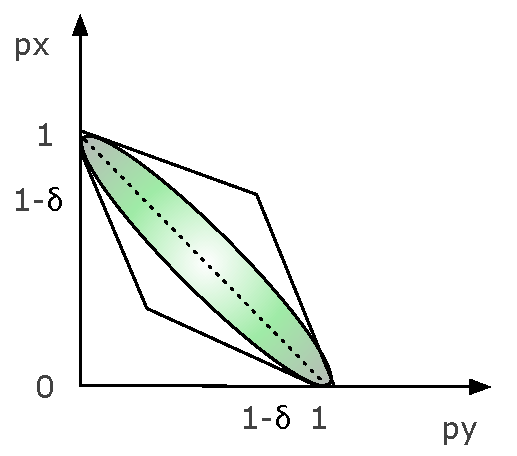
\includegraphics[width=2.5in]{fig/privacyregion.pdf}
\caption{\label{privacy_region} Every tangent line of the privacy region forms a pair of $(\epsilon, \delta)$. }
\end{figure}
As it is shown in Figure~\ref{privacy_region}, every tangent line of the privacy region corresponds to a pair of $(\epsilon, \delta)$. In general, the privacy region $R(M, x, x')$ of any mechanism $M$ can be represented by the intersections of all such regions $\{R(\epsilon_{i}, \delta_{i})\}$, which is completely described by the set of slopes and shifts $\{(\epsilon_{i}, \delta_{i})\}$.
\begin{enumerate}
\item For the set slopes, let ${\cal E} = \{0 \leq \epsilon_{i} < \infty \,|\, Pr[M(x)=y] = e^{\epsilon_{i}}Pr[M(x')=y] \text{ for some $y \in {\cal Y}$} \}$
\item For each $\epsilon_{i}$,  $\delta_{i} = \max_{S \subseteq {\cal Y}} \{ \Sigma_{y \in S}Pr[M(x)=y] - e^{\epsilon_{i}}\Sigma_{y \in S}Pr[M(x)=y]\}$
\end{enumerate}
\subsection{Case of CW-P}
In the case of CW-P, we use $X$ to denote a database variable that follows some distribution $D$. Let the pmf of $D$ be $f_{D} =[{f_{x_{1}} , \dots, f_{x_{n}}}]$. Let $alt(X)$ denote a scrubbed version of $X$. Assume $alt(X)$ follows some distribution $D'$ with pmf $f'_{D}$.

It is easy to see that CW-P has the following equivalent definition.
\begin{theorem}
For any $\epsilon \geq 0$ and $\delta \in [0, 1]$, a mechanism $M$ is $(\epsilon, \delta,\Delta, \Gamma)$-differentially private if and only if the following conditions are satisfied for all distributions on $D$ on $(X, Z)$, all $(priv, alt) \in \Gamma$ pairs, and all region $S \subseteq {\cal Y}$:
\[
Pr[M(X) \in S \,|\, priv(X), Z]+e^{\epsilon}Pr[M(alt(X)) \in \bar{S}\,|\, priv(X), Z] \geq 1-\delta , \quad and
\]
\[
e^{\epsilon}Pr[M(X) \in S\,|\, priv(X), Z]+Pr[M(alt(X)) \in \bar{S}\,|\, priv(X), Z]  \geq 1-\delta ,
\]
where $M(X) = f_{D}M$ and $M(alt(X))=f'_{D}M$.
\end{theorem}
Notice mechanism $M' = [f_{D}M, f'_{D}M]^{\top}$ can be seen as a DP version of $M$. Hence, CW-P also has form of privacy regions, and everything else described above follows.
\section{Composition Theorem of CW-P in the streaming setting}
\begin{figure}[th]
\centering
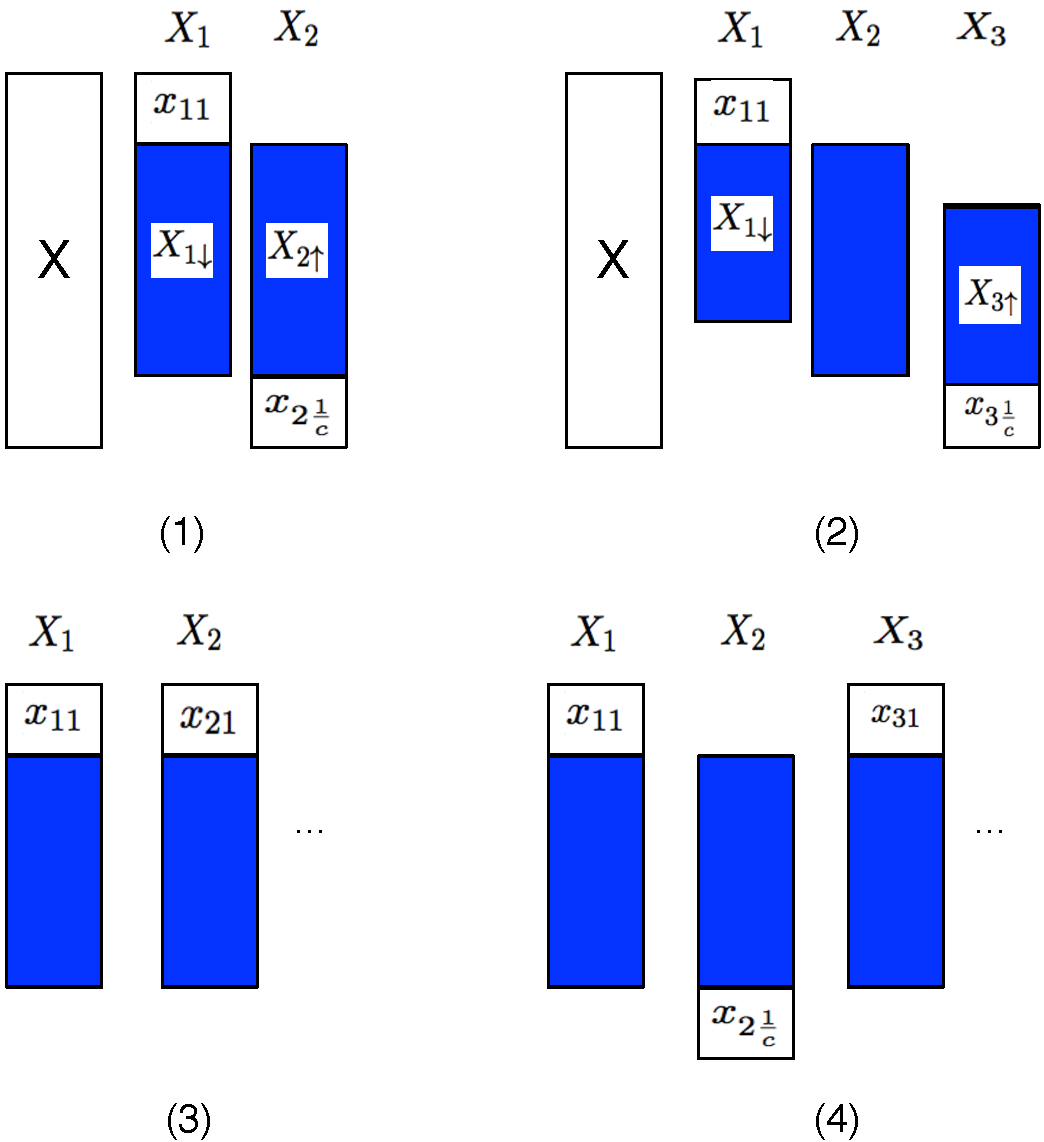
\includegraphics[width=4.8in]{fig/stream_database1.pdf}
\caption{\label{stream_db1} Blocks in blue are shared by more than one databases. Blocks in white are owned by only one database. (1) Composition of $F(X_{1})$ and $F(X_{2})$. It has ``good" independence since each $X_{i}$ owns one block. (2) Composition of queries on three streaming databases. Cannot leverage ``good" independence, because each block in $X_{2}$ is shared by two databases. (3) Composition of queries in the standard DP case. The blue blocks refer to the query while the white blocks refer to the independent noise. (4) It works as long as each streaming database owns one block of ``private" block.}
\end{figure}
{\bf Problem setting} \\
Let $X$ be a database in the streaming setting. Let $X_{i}$ represent the portion of $X$ that is currently held at time step $i$. We assume that at each time step, a fraction of $c$ of the database is replaced. We assume the oldest rows are always the ones replaced, and that $X$ has row drown i.i.d. from some distribution $D$. Let $n$ be the size of each $X_{i}$. This means that the first $n$ rows of $X$ constitute $X_{1}$, rows $cn+1$ through $cn+n$ constitute $X_{2}$, and so forth. $X$ has size $n+cn(t-1)$, where $t$ is the total number of time steps being considered. $1/c$ is the total number of time steps a given row will be present for. See (1) and (2) in Figure~\ref{stream_db1}. 
\\
\\
{\bf Notations and definitions}\\
For each $X_i$ of size $n$, we represent it by $1/c$ blocks (each has $cn$ rows). Namely, let $X_{i}=\xblock{i}$, where $x_{ij}$ denote the $j$th block in $X_{i}$. Let $\xdown{i} = [x_{i 2} , \dots, x_{i \frac{1}{c}}]^{\top}$ and $\xup{i} = [x_{i 1}, x_{i2} , \dots, x_{i (\frac{1}{c}-1)}]^{\top}$. Namely, $\xdown{i}$ represent the bottom $(1/c -1)$ blocks of $X_{i}$ while $\xup{i}$ represent the top $(1/c-1)$ blocks of $X_{i}$.

Consider a mechanism $M: \, {\cal X} \rightarrow {\cal Y}$, where ${\cal X} = \{x_{1}, \dots , x_{n}\}$ and ${\cal Y}=\{y_{1}, \dots , y_{m}\}$. (We assume $\cal X$ and $\cal Y$ are finite discrete for the simplicity of analysis.). $M$'s auxiliary information consists of {\bf the last $(1-c)n$ rows} of the database $X_{i}$, i.e., $\xdown{i}$ is given. 
\\
\\
{\bf Assumptions}
\begin{enumerate}
\item We assume that there is a subset ${\cal W} \subseteq {\cal Y}$ such that (we ignore the $priv(X_{i})$ in the expression)
\begin{enumerate}
\item $\forall y \in {\cal W},\, \forall z: \conpr{M(X_{i})=y}{\xdown{i}=z} \neq 0 \text{ , }\conpr{M(alt(X_{i}))=y}{\xdown{i}=z} \neq 0$ ;
\item $\forall y \in {\cal Y-W},\, \forall z: \conpr{M(X_{i})=y}{\xdown{i}=z} = 0 \text{ , }\conpr{M(alt(X_{i}))=y}{\xdown{i}=z} = 0$ .
\end{enumerate}
\item According to section 1, $M$ can be characterized as a convex region. It should have a set of $(\epsilon_{j}, \delta_{j})$, whose values are computable by the slope and shift of the tangent lines of $M$ on some $y_{j}$. For each $y_{j} \in {\cal W}$ and for all $z$, we denote the slope of the tangent line on $y_{j}$ as 
\begin{equation}
 e^{\epsilon_{j|z}} = \frac{\conpr{M(X_{i})=y_{j}}{\xdown{i}=z} }{\conpr{M(alt(X_{i}))=y_{j}}{\xdown{i}=z} } \geq  1.
\end{equation}
It's corresponding shift $\delta_{j|z}$ is the follows.
\begin{equation}
\delta_{j|z} =\max_{S \subseteq {\cal W}} \{ \Sigma_{y \in S}\conpr{M(X_{i})=y_{j}}{\xdown{i}=z} - e^{\epsilon_{j|z}}\Sigma_{y \in S}\conpr{M(alt(X_{i}))=y_{j}}{\xdown{i}=z}\} 
\end{equation} 
For each $z$, let $\epsilon_{z|min} = \min_{j} \{\epsilon_{j|z} \}$ and $\epsilon_{z|max}= \max_{j} \{\epsilon_{j|z} \}$. Obviously, the minimal shift $\delta_{z|min} $ is computed by $\epsilon_{z|max}$. The maximal shift $\delta_{z|max} $ is computed by $\epsilon_{z|min}$. Let $\epsilon_{max} = \max_{z} \{\epsilon_{z|max}\}$ and $\delta_{max} = \max_{z} \{\delta_{z|max}\}$.

Let ${\cal E} = \{(\epsilon_{j|z}, \delta_{j|z})\}$ be the set of all slope-shift pairs. Then, $M$ is $(\epsilon, \delta, \Delta, \Gamma)$-CW private is  CW-private for all $(\epsilon, \delta) \in {\cal E}$, where $\Delta$ specifies the distribution on $X_{i}$ and the auxiliary information as stated above.
\item For each $y_{j} \in {\cal W}$, we assume the following bound.
\begin{equation}
\forall z, z', \, \frac{\conpr{M(X_{i})=y_{j}}{\xdown{i}=z} }{\conpr{M(alt(X_{i}))=y_{j}}{\xdown{i}=z'} } \leq e^{\gamma_{j}},
\end{equation}
where $\gamma_{j}>0$ is a small constant. We denote $\gamma = \max_{j} \{\gamma_{j}\}$.
\end{enumerate}
{\bf Additional notations. } For the simplicity of the proofs, we use $P^{0}(y_{1}, \dots , y_{t} \,|\, z)$ to denote $\conpr{M(X_{1})=y_{1}, \dots M(X_{t})=y_{t}}{\xdown{t}=z} $, and use $P^{1}(y_{1}, \dots , y_{t} \,|\, z)$ to denote $\conpr{M(alt(X_{1}))=y_{1}, \dots M(alt(X_{t}))=y_{t}}{\xdown{t}=z'} $. 
\begin{lemma}
For any $[y_{1}, \dots , y_{t}] \in {\cal W}^{t}$, we have the following bound
\[
\forall z, z', \, \frac{\po{t}{z} }{\pl{t}{z'}} \leq e^{\Sigma_{j=1}^{t}\gamma_{j}}
\]
\end{lemma}
{\bf Proof.} We prove this inductively. The base case is trivially true. Assume the lemma is true for $t-1$. For any $z, z'$, conditioned on the first block of $X_{t}$ (i.e., $X_{t1}$ ), we have
\[
\frac{\po{t}{z} }{\pl{t}{z'}} 
\]
\[
 = \frac{\Sigma_{z*}\po{t-1}{X_{t1}=z*, \xdown{t}=z} \pos{t}{X_{t1}=z*, \xdown{t}=z} Pr[X_{t1}=z*]}{\Sigma_{z*}\pl{t-1}{X_{t1}=z*, \xdown{t}=z'} \pls{t}{X_{t1}=z*, \xdown{t}=z'} Pr[X_{t1}=z*]}
\]
\[
=\frac{\Sigma_{z*}\po{t-1}{[z*,z]_{\uparrow}} \pos{t}{X_{t}=[z*,z]} Pr[X_{t1}=z*]}{\Sigma_{z*}\pl{t-1}{[z*,z']_{\uparrow}} \pls{t}{X_{t}=[z*,z']} Pr[X_{t1}=z*]}
\]
where $[z*,z]_{\uparrow}$ denote the top (1/c -1) blocks of database $[z*, z]$.
\[
\leq \max_{z_{1}, z_{2}} \{ \frac{\po{t-1}{z_{1}}}{\pl{t-1}{z_{2}}} \} \cdot \frac{\Sigma_{z*}\pos{t}{X_{t}=[z*,z]} Pr[X_{t1}=z*]}{\Sigma_{z*}\pls{t}{X_{t}=[z*,z']} Pr[X_{t1}=z*]}
\]
\[
\leq e^{\Sigma_{j=1}^{t-1} \gamma_{j}} \cdot \frac{\Sigma_{z*}\pos{t}{X_{t}=[z*,z]} Pr[X_{t1}=z*]}{\Sigma_{z*}\pls{t}{X_{t}=[z*,z']} Pr[X_{t1}=z*]}
\]
\[
= e^{\Sigma_{j=1}^{t-1}\gamma_{j}} \cdot \frac{\pos{t}{z}}{ \pls{t}{z'}} \leq e^{\Sigma_{j=1}^{t}\gamma_{j}} \quad \blacksquare
\]
\begin{lemma}\label{slope_bound}
Let $G(X) = (M(X_{1}), M(X_{2}) , \dots, M(X_{t}))$ be the composite query that runs $M$ at each time step. The slope of $G$ on $[y_{1}, \dots , y_{t}] \in {\cal W}^{t}$ has the following bound.
\[
\forall z, \frac{\po{t}{z}}{\pl{t}{z}} \leq e^{\Sigma_{j=1}^{t-1}\gamma_{j} + \epsilon_{t|z}}
\]
\end{lemma}
{\bf Proof.} For any $z$, we have
\[
\frac{\po{t}{z}}{\pl{t}{z}} = \frac{\Sigma_{z*} \po{t-1}{[z*,z]_\uparrow} \pos{t}{X_{t}=[z*,z]} Pr[X_{t1}=z*]}{\Sigma_{z*} \pl{t-1}{[z*,z]_\uparrow} \pls{t}{X_{t}=[z*,z]}Pr[X_{t1}=z*]}
\] 
\[
\leq \max_{z_{1}, z_{2}} \{ \frac{\po{t-1}{z_{1}}}{\pl{t-1}{z_{2}}} \} \cdot \frac{\Sigma_{z*}\pos{t}{X_{t}=[z*,z]} Pr[X_{t1}=z*]}{\Sigma_{z*}\pls{t}{X_{t}=[z*,z]} Pr[X_{t1}=z*]}
\]
\[
= e^{\Sigma_{j=1}^{t-1}\gamma_{j}} \cdot \frac{\pos{t}{z}}{ \pls{t}{z}} = e^{\Sigma_{j=1}^{t-1}\gamma_{j} + \epsilon_{j|z}} \quad \blacksquare
\]

\begin{theorem}
Let $G(X) = (M(X_{1}), M(X_{2}) , \dots, M(X_{t}))$ be the composite query that runs $M$ at each time step. Then, $G$ is $( \epsilon_{t},  \delta_{t}, \Delta, \Gamma)$ -CW private, where $ \epsilon_{t} \leq \epsilon_{max} + (t-1)\gamma$ and $\delta_{t} \leq t \delta_{max}$. 
\end{theorem}
{\bf Proof.} Pick $\epsilon_{t}$ that corresponds to the largest slope on $G$. By Lemma~\ref{slope_bound}, it is easy to see $\epsilon_{t} \leq \epsilon_{max} + (t-1)\gamma$. Next, we prove shift part of the theorem inductively. Notice that when $\epsilon_{t}$ is the largest slope on $G$, we have
\[
\delta_{t} = \max_{S \subseteq {\cal W}^{t}} \{\Sigma_{[y_{1}, \dots ,y_{t}]\in S} \po{t}{z} - e^{\epsilon_{t|z}}\Sigma_{[y_{1}, \dots ,y_{t}]\in S} \pl{t}{z}\}
\]
\[
=\Sigma_{[y_{1}, \dots ,y_{t}]: \pl{t}{z}=0} \po{t}{z}
\]
\[
=1- \Sigma_{[y_{1}, \dots ,y_{t}]\in S_{t}} \po{t}{z}
\]
where $S_{t}=\{[y_{1}, \dots ,y_{t}] \,|\, \pl{t}{z}\neq 0 \}$. Notice that
\[
\pl{t}{z} = \Sigma_{z*} \pl{t-1}{[z*,z]_\uparrow} \pls{t}{X_{t}=[z*,z]}Pr[X_{t1}=z*]
\]
From now on, we only consider $z*$ with $Pr[X_{t1}=z*] \neq 0$.

Let $V_{t-1|z*} = \{[y_{1}, \dots ,y_{t-1}] \,|\,  \pl{t-1}{[z*,z]_\uparrow} \neq 0  \}$. Let $V_{t|z*} =\{y_{t} \,|\, \pls{t}{X_{t}=[z*,z]} \neq 0\}$. Obviously, we have $V_{t-1|z*} \times V_{t|z*} \subseteq S_{t}$ for all $z*$. 

We next show the lower bound of $\Sigma_{[y_{1}, \dots ,y_{t}]\in S_{t}} \po{t}{z} $.
\[
\Sigma_{[y_{1}, \dots ,y_{t}]\in S_{t}} \po{t}{z} 
\]
\[
= \Sigma_{[y_{1}, \dots ,y_{t}]\in S_{t}} \Sigma_{z^{\#}} \po{t-1}{[z^{\#}, z]_\uparrow} \pos{t}{X_{t}=[z^{\#}, z]} Pr[X_{t1}=z^{\#}]
\]
\[
\geq \Sigma_{z^{\#}} \Sigma_{[y_{1}, \dots ,y_{t}] \in V_{t-1|z^{\#}} \times V_{t|z^{\#}} } \po{t-1}{[z^{\#}, z]_\uparrow} \pos{t}{X_{t}=[z^{\#}, z]} Pr[X_{t1}=z^{\#}]
\]
\[
=\Sigma_{z^{\#}} \Sigma_{y_{t} \in V_{t|z^{\#}}}\Sigma_{[y_{1}, \dots ,y_{t-1}] \in V_{t-1|z^{\#}} } \po{t-1}{[z^{\#}, z]_\uparrow} \pos{t}{X_{t}=[z^{\#}, z]} Pr[X_{t1}=z^{\#}]
\]
By the inductive hypothesis, 
\[
\geq \Sigma_{z^{\#}} \Sigma_{y_{t} \in V_{t|z^{\#}}}  (1- (t-1)\delta_{max}) \pos{t}{X_{t}=[z^{\#}, z]} Pr[X_{t1}=z^{\#}]
\]
\[
= (1- (t-1)\delta_{max})  \Sigma_{z^{\#}} \Sigma_{y_{t} \in V_{t|z^{\#}}} \pos{t}{X_{t}=[z^{\#}, z]} Pr[X_{t1}=z^{\#}]
\]
Let $V_{t}= \{y_{t} \,| \, \pls{t}{z} \neq 0\}$. Then, we have
\[
=(1- (t-1)\delta_{max})  \Sigma_{y_{t} \in V_{t}} \pos{t}{ z} 
\]
Since $\Sigma_{y_{t} \in V_{t}} \pos{t}{ z} $ is the minimum shift value of $M(X_{t})$ given $\xdown{t}=z$, we have
\[
\geq (1- (t-1)\delta_{max}) (1- \delta_{z|min})\geq 1 - t\delta_{max}.
\]
It follows that 
\[
\delta_{t} = 1- \Sigma_{[y_{1}, \dots ,y_{t}]\in S_{t}} \po{t}{z} \leq t\delta_{max}. \quad \blacksquare
\]

\end{document}
